% 图 1 首图：跨栏，由 manuscript_zh.tex 以 \twocolumn[{...}] 置于标题下方。
% 选定三栏底稿（2026-11-03）：figures/Fig1/INDEX.md。
\begin{center}
\captionsetup{type=figure}
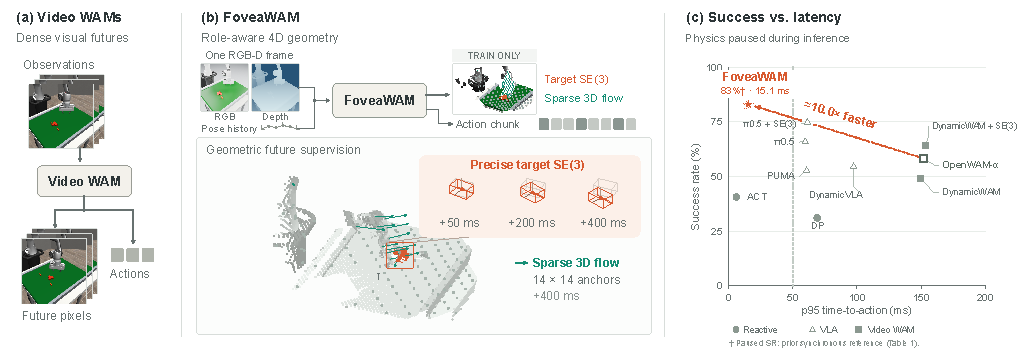
\includegraphics[width=\textwidth]{figures/Fig1/fig1.pdf}
\captionof{figure}{\textbf{\ours 按任务角色分配预测精度。}(a) 用参考录制展示稠密视频未来预测及动作输出的表示形式。(b) \ours 以一帧 RGB-D 和位姿历史为条件。目标 SE(3) 与稀疏 3D 流只用于训练监督，部署时输出动作块。裁切点云展示当前参考几何；未来位姿与流均为真实监督标签，并非模型预测。流在 \cfgContextGrid{} 网格上采样；箭头表示放大 $3\times$ 的 400\,ms 位移。位姿字形展示 $+50$、$+200$ 和 $+400$\,ms 时的目标。(c) 表~\ref{tab:main} 的 Paused 成功率（推理期间暂停物理）与原生 p95 出动作时间。虚线标记 50\,ms。\ours 星形点（83\%、28\,ms）及相对 OpenWAM-$\alpha$（151.7\,ms）的 $\approx5.4\times$ 加速均为排版占位，尚待实测。}
\label{fig:teaser}
\end{center}
